\documentclass[conference]{IEEEtran}
\IEEEoverridecommandlockouts

\usepackage{cite}
\usepackage{amsmath,amssymb,amsfonts}
\usepackage{graphicx}
\usepackage{textcomp}
\usepackage{xcolor}
\usepackage{booktabs}
\usepackage{array}
\usepackage{url}

% Float placement optimization
\renewcommand{\topfraction}{0.95}
\renewcommand{\bottomfraction}{0.95}
\renewcommand{\textfraction}{0.05}
\renewcommand{\floatpagefraction}{0.85}
\renewcommand{\dbltopfraction}{0.95}
\renewcommand{\dblfloatpagefraction}{0.85}

\newcommand{\deployfunc}{\textsf{switch\allowbreak\_to\allowbreak\_deploy}}

\def\BibTeX{{\rm B\kern-.05em{\sc i\kern-.025em b}\kern-.08em
    T\kern-.1667em\lower.7ex\hbox{E}\kern-.125emX}}

\begin{document}

\title{Structural Re-Parameterization, Spatial Coordinate Encoding, and Cross-Domain Robustness for Real-Time Safety Helmet Detection in Construction Surveillance\thanks{This research is supported by FPT University. This paper is prepared for presentation at the 2027 2nd International Conference on Advances in Artificial Intelligence and Machine Learning (AAIML 2027), Tokyo, Japan. Corresponding author: Nhu Han (email: nhu.han@fpt.edu.vn).}}

\author{
\IEEEauthorblockN{Nhu Han\IEEEauthorrefmark{1}, Van-Thanh Nguyen\IEEEauthorrefmark{1}, Tuan-Dung Nguyen\IEEEauthorrefmark{1}, and Hai-Anh Vu\IEEEauthorrefmark{2}}
\IEEEauthorblockA{\IEEEauthorrefmark{1}Department of Artificial Intelligence, FPT University, Hanoi, Vietnam\\
\IEEEauthorrefmark{2}Department of Information Technology, FPT University, Hanoi, Vietnam\\
Email: \{nhu.han, thanhnv, dungnt\}@fpt.edu.vn, anhvh@fe.edu.vn}
}

\maketitle

\begin{abstract}
Automated Personal Protective Equipment (PPE) compliance monitoring via closed-circuit television (CCTV) feeds is vital for injury prevention on dynamic construction sites. However, practical edge surveillance encounters severe operational bottlenecks, including distant tiny helmet targets (under 20x20 pixels), extreme class imbalance (up to a 1:12 helmet-to-person ratio), multi-scale occlusions, and background clutter. In this paper, we present Rep-YOLO11s, a domain-specialized, latency-optimized real-time object detection framework tailored for complex industrial surveillance. Rather than claiming isolated module inventions, Rep-YOLO11s contributes a principled architectural integration of four established mechanisms: (1) Structural Re-parameterization (RepConv) multi-branch training blocks algebraically folded into single 3x3 convolutions at inference for zero deployment overhead; (2) Spatial Coordinate Convolution (CoordConv) injected strictly at the initial Stem layer to supply vertical spatial inductive priors at negligible latency (+0.06 ms); (3) Bi-Level Routing Attention (BiFormer, S=8, k=4) in neck feature maps to dynamically route compute toward distant helmet contours while pruning 93.75 percent of irrelevant background tokens; and (4) Focal EIoU Loss for bounding box regression, which decomposes aspect ratio penalties into independent Euclidean distances and weights hard localization samples, while class and candidate imbalance are resolved via Task-Aligned Assignment (TAL) and aligned classification loss. Benchmark evaluations on the Safety Helmet Wearing Dataset (SHWD / VOC2028) show that Rep-YOLO11s achieves 94.83 percent mAP50 and 62.54 percent mAP50-95, with 5-fold cross-validation reaching a mean mAP50 of 96.64 percent (standard deviation 0.32 percent, peak 97.11 percent). In deployment audits, batch-one TensorRT FP16 execution at 640x640 achieves 2.92 ms (342.5 FPS) on NVIDIA Tesla T4, 5.35 ms (187.1 FPS) on RTX 3050 Laptop GPU, and real-time execution on an entry-level GeForce MX230 (36.0 ms, 27.8 FPS). Zero-shot evaluations across diverse external industrial datasets (GDUT-HWD, Hard Hat Workers, and SHD) confirm robust cross-domain transferability under harmonized PPE evaluation protocols.
\end{abstract}

\begin{IEEEkeywords}
Safety Helmet Detection, Structural Re-parameterization, Bi-Level Routing Attention, CoordConv, Focal EIoU Loss, Cross-Domain Generalization, Real-Time Edge AI, Construction Surveillance.
\end{IEEEkeywords}

\section{Introduction}
Personal Protective Equipment (PPE) compliance monitoring, particularly for safety helmets, is strictly mandated across industrial construction sites to prevent traumatic head injuries. While automated intelligent video analytics via CCTV streams offer continuous, non-intrusive compliance auditing, deploying computer vision models in real-world construction environments encounters four major operational bottlenecks:
\begin{enumerate}
    \item \textbf{Distant Tiny Targets}: Long-range CCTV cameras positioned at high elevations render helmets as sub-$20\times20$ pixel targets subject to severe feature attenuation across deep convolutional backbones.
    \item \textbf{Severe Class Imbalance}: Industrial benchmarks like the Safety Helmet Wearing Dataset (SHWD) exhibit acute category skew ($9,044$ helmet vs. $111,514$ person instances, a $1:12$ ratio), biasing standard losses toward background and torso features.
    \item \textbf{Spatial Distractor Confusion}: Construction sites abound with visually confusing round objects (yellow buckets, orange traffic cones, warning signage) that trigger false alarms under standard translation-invariant convolutions lacking vertical context.
    \item \textbf{Strict Edge Latency Bounds}: Multi-camera edge monitoring demands real-time throughput ($\ge 60$ FPS), penalizing complex attention mechanisms with prohibitive memory access costs (MAC) and kernel launch overheads.
\end{enumerate}

To overcome these barriers in a unified framework, we present \textbf{Rep-YOLO11s}. Our scientific contribution lies in the principled architectural integration and latency-optimized deployment lifecycle of proven mechanisms tailored specifically for industrial surveillance:
\begin{itemize}
    \item \textbf{RepConv Structural Fusion}: Multi-branch training topologies ($3\times3$, $1\times1$, and identity strictly guarded by $\mathbb{I}_{\{C_{in}=C_{out} \land s=1\}}$) fold algebraically into single $3\times3$ kernels (\deployfunc) for inference, eliminating residual memory buffers for zero deployment overhead.
    \item \textbf{Stem CoordConv}: Normalized coordinates $(x, y) \in [-1, 1]$ injected strictly at the initial Stem layer ($5 \to 64$) supply vertical spatial inductive priors at negligible cost (+0.06~ms), enabling the network to differentiate head-worn helmets from ground distractors.
    \item \textbf{BiFormer Token Routing}: Dynamic bi-level routing attention ($S=8, k=4$) in neck stages ($P_4, P_5$) filters out $93.75\%$ of irrelevant background tokens, focusing representation on tiny helmet contours with minimal runtime overhead (+0.24~ms).
    \item \textbf{Decoupled Imbalance \& Loss}: Focal EIoU bounding-box regression ($\gamma=0.5$) resolves aspect ratio gradient vanishing, while category imbalance is decoupled and handled via Task-Aligned Assignment (TAL) and aligned classification loss ($\mathcal{L}_{cls}$).
    \item \textbf{Empirical SOTA \& Deployment Parity}: Tested across SHWD (94.83\% $mAP_{50}$; 5-fold CV 96.64\%) and five external datasets. Benchmarked with strict stream synchronization across Tesla T4 (2.92~ms TRT FP16), RTX 3050 Laptop (5.35~ms TRT FP16), and entry-level MX230 (36.0~ms / 27.8~FPS).
\end{itemize}

%-------------------------------------------------------------------------
\section{Related Work}
\label{sec:related}

\subsection{Real-Time Object Detection Frameworks}
Real-time single-stage object detection has evolved through the YOLO series~\cite{wang2023yolov7,wang2024yolov10,ultralytics2024yolo11}. YOLOv6~\cite{li2023yolov6} pioneered structural re-parameterization via EfficientRep backbones and Rep-PAN. YOLOv8 introduced anchor-free C2f modules, while YOLOv10~\cite{wang2024yolov10} developed dual-assignment NMS-free training. Ultralytics YOLO11~\cite{ultralytics2024yolo11} refined feature pyramid alignment via C3k2 and C2PSA blocks. However, general detectors lack domain-specific mechanisms to handle tiny targets, severe class skew, and spatial distractor confusion.

\subsection{Safety Helmet Detection in Complex Environments}
Specialized architectures have tailored detectors for PPE auditing. EC-YOLOv8~\cite{ecyolov8_2024} incorporated ECA attention, CARAFE upsampling, and EIoU loss into YOLOv8n, reporting $95.7\%$ $mAP_{50}$ on SHWD; however, CARAFE reduces speed to $172\text{~FPS}$ on desktop GPUs, and the model remains sensitive to color-confused background objects. Wu \textit{et al.}~\cite{yolocbf_2025} proposed YOLO-CBF combining CoordConv, BiFormer attention, and Focal-EIoU, achieving gains on a small 962-image road dataset without validating against industrial clutter or class skew. Zhao \textit{et al.}~\cite{zhao2025yolodcrcf} introduced YOLO-DCRCF based on YOLO11 with Deformable Convolution (DCNv2) and recalibrated feature pyramids (RCF) for power-grid inspection; however, DCNv2 incurs irregular memory access that penalizes TensorRT execution. Song \textit{et al.}~\cite{song2024improved} proposed an improved YOLOv8 combining Dilated Residual Wavelet (DWR) modules, ASPP, and NWD loss, but parallel dilated branches expand memory footprint. Additional variants including DABFNet~\cite{dabfnet2024}, MAF-YOLO~\cite{mafyolo2024}, and YOLOv8n-FADS~\cite{fuYolov8nFADSStudyEnhancing2024} either incur quadratic attention overhead or fail to decouple multi-branch training topologies from edge execution kernels.

\subsection{Structural Re-parameterization and Spatial Encoding}
Structural re-parameterization, pioneered by RepVGG~\cite{ding2021repvgg} and adopted in YOLOv6~\cite{li2023yolov6}, decouples training representation from inference execution. Parallel branches ($3\times3$, $1\times1$, identity) provide gradient diversity during backpropagation and are algebraically folded into single $3\times3$ convolutions at deployment, eliminating residual branching and reducing Memory Access Cost (MAC). CoordConv~\cite{liu2018coordconv} breaks translation equivariance by concatenating coordinate channels, providing vertical spatial priors critical for distinguishing helmets on human heads from ground-level construction materials.

%-------------------------------------------------------------------------
\section{Proposed Methodology}
\label{sec:method}

\begin{figure}[t]
\centering
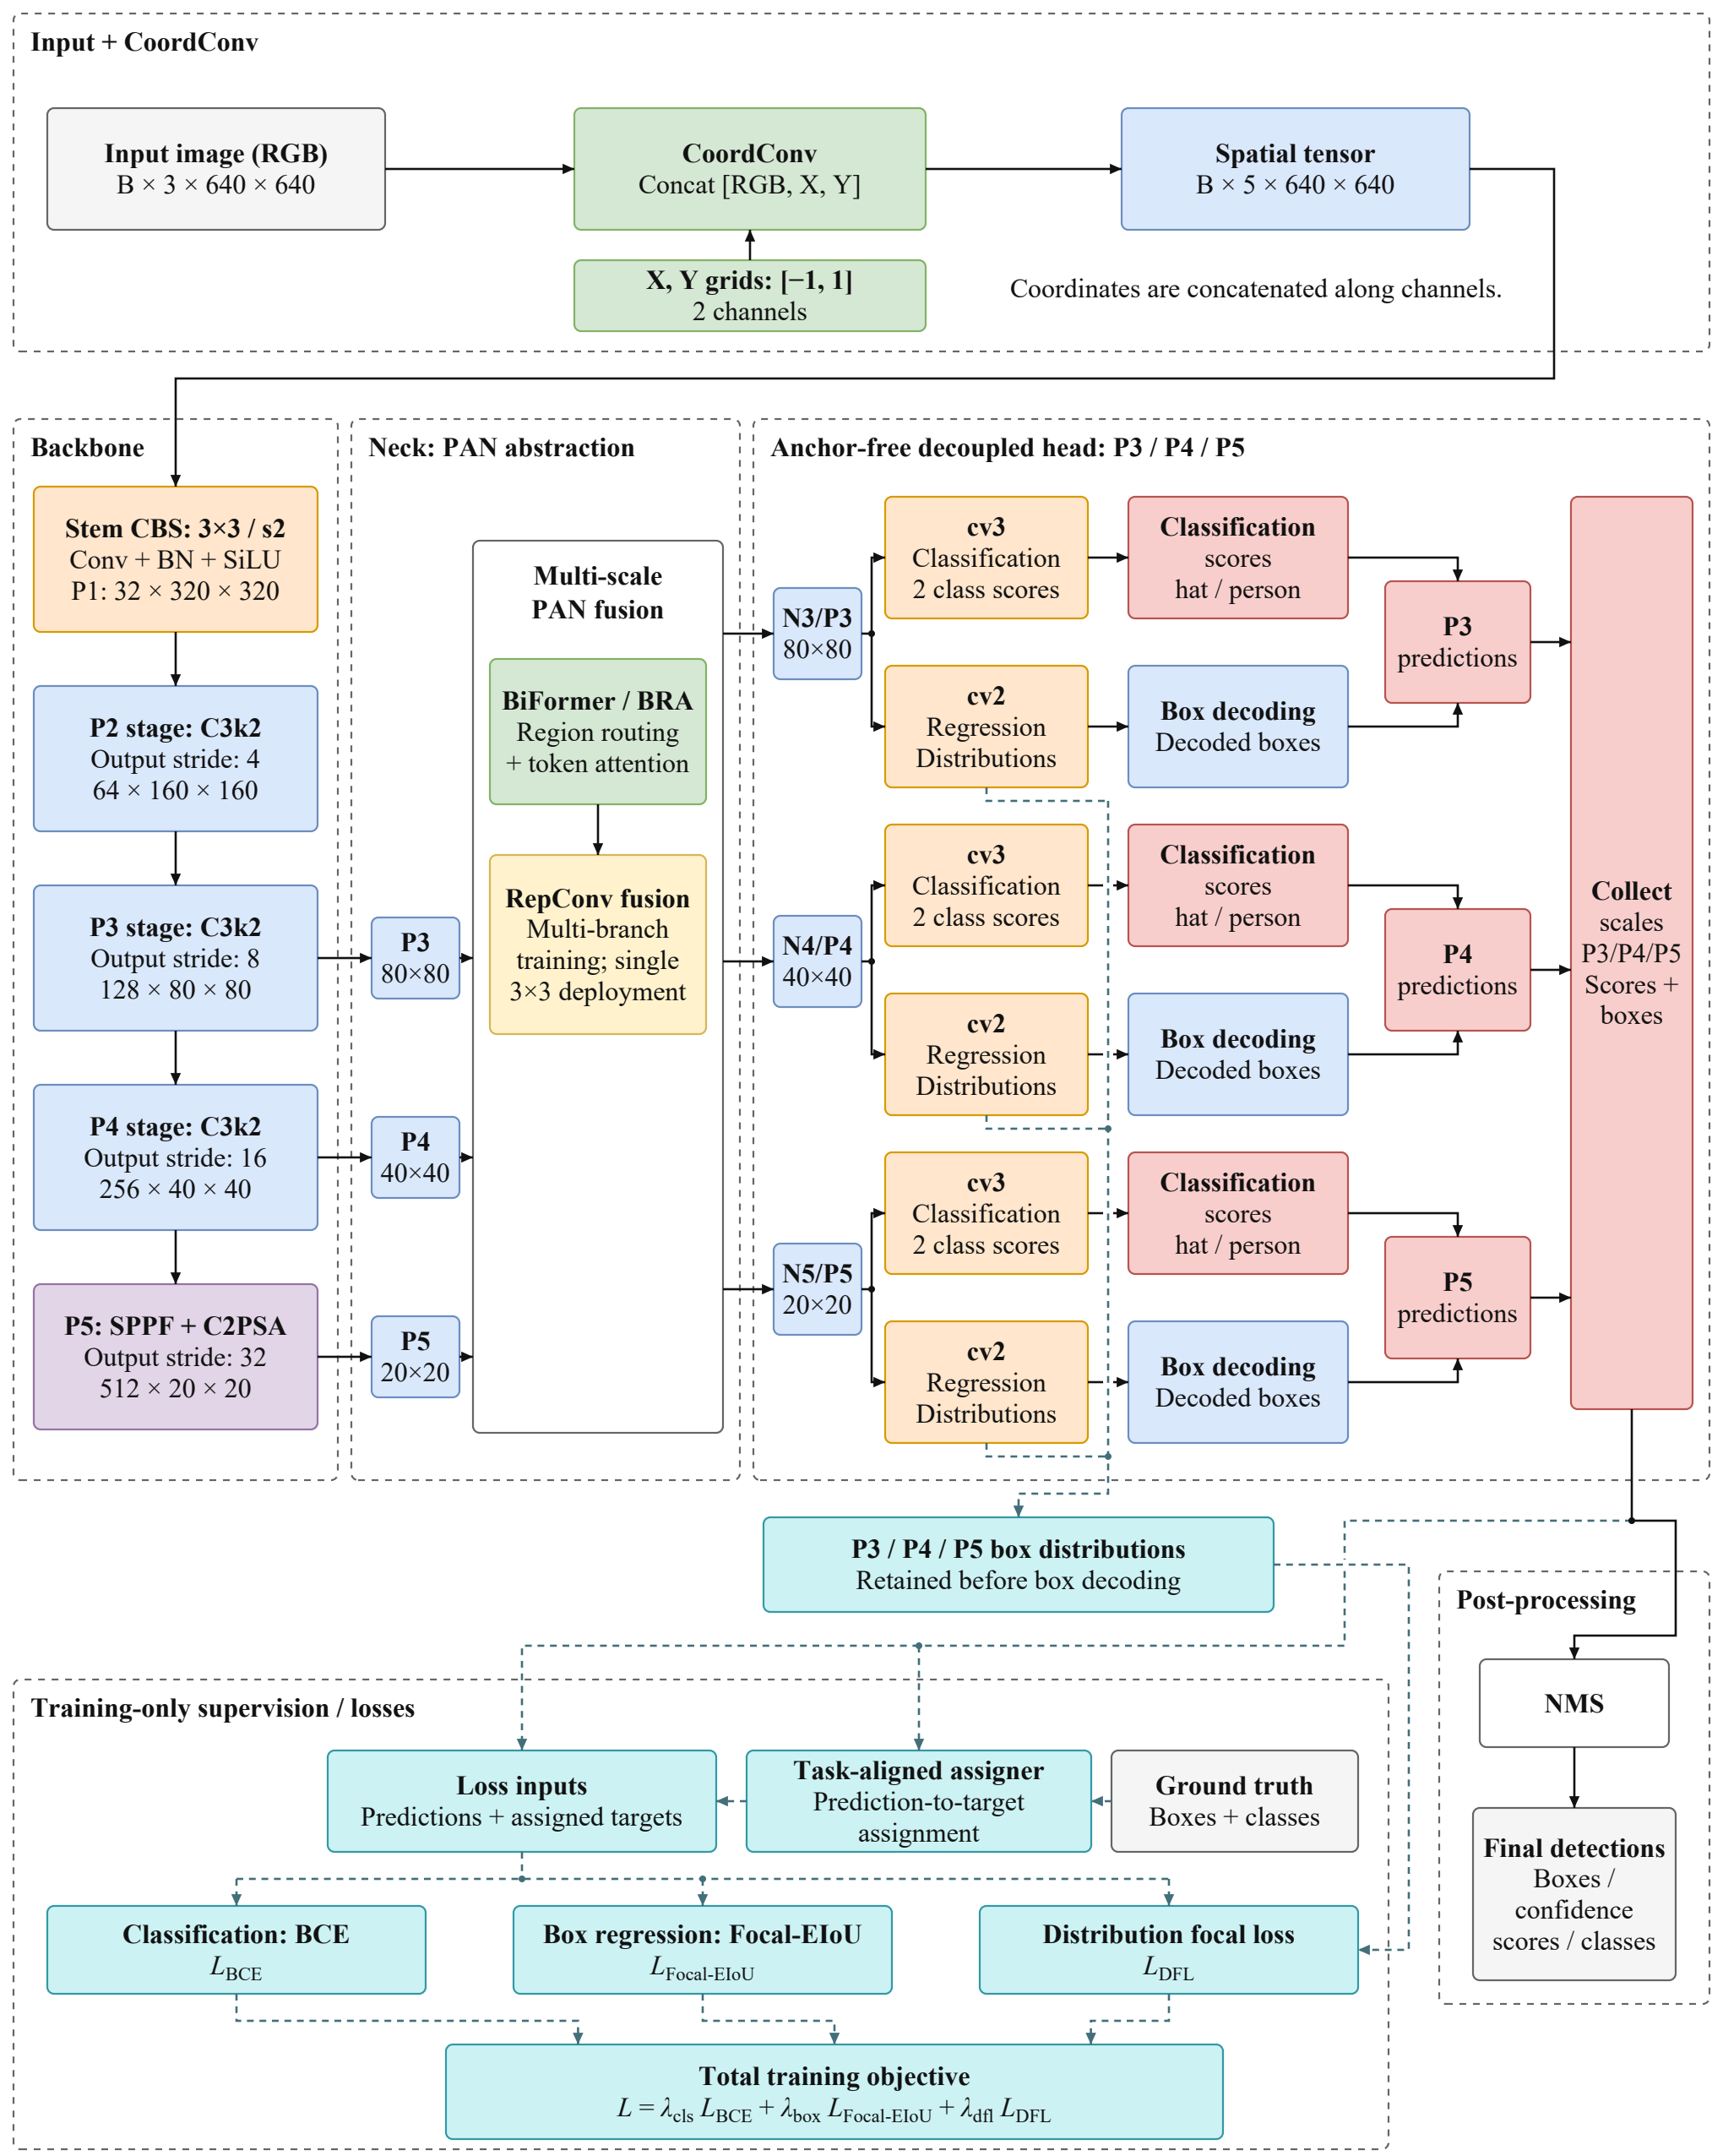
\includegraphics[width=\columnwidth]{figures/rep_yolo11s_overall_ieee.png}
\caption{Overall Architecture of Rep-YOLO11s. The pipeline integrates: (1) Stem CoordConv coordinate concatenation ($[RGB, X, Y] \to 5\times640\times640$); (2) Multi-scale backbone feature extraction (P1 Stem, P2--P4 C3k2, P5 SPPF+C2PSA); (3) PAN neck abstraction with Bi-Level Routing Attention (BRA) and RepConv; (4) Anchor-free decoupled detection heads (P3, P4, P5) predicting classification logits ($cv3$) and distribution regression ($cv2$); and (5) Multi-task loss supervision with Task-Aligned Assigner (TAL), BCE, Focal-EIoU, and DFL.}
\label{fig:architecture_overview}
\end{figure}

\subsection{Overall System Architecture}
The architecture of Rep-YOLO11s is illustrated in Fig.~\ref{fig:architecture_overview}. The framework adopts an end-to-end single-stage design developed from Ultralytics YOLO11~\cite{ultralytics2024yolo11}, comprising: (1) a Structural Re-parameterized Backbone enhanced with Stem CoordConv; (2) a Path Aggregation Network (PAN) Neck~\cite{lin2017feature,liu2018path} integrated with BiFormer Bi-Level Routing Attention; and (3) an Anchor-Free Decoupled Detection Head trained with Focal EIoU Bounding Box Loss and Task-Aligned Assignment.

\subsection{Structural Re-parameterization (RepConv) Mechanics}
To achieve high non-linear feature representation during training without incurring latency penalties during edge deployment, RepConv blocks are embedded within critical neck aggregation pathways.

\begin{figure*}[t]
\centering
\begin{minipage}[b]{0.49\textwidth}
  \centering
  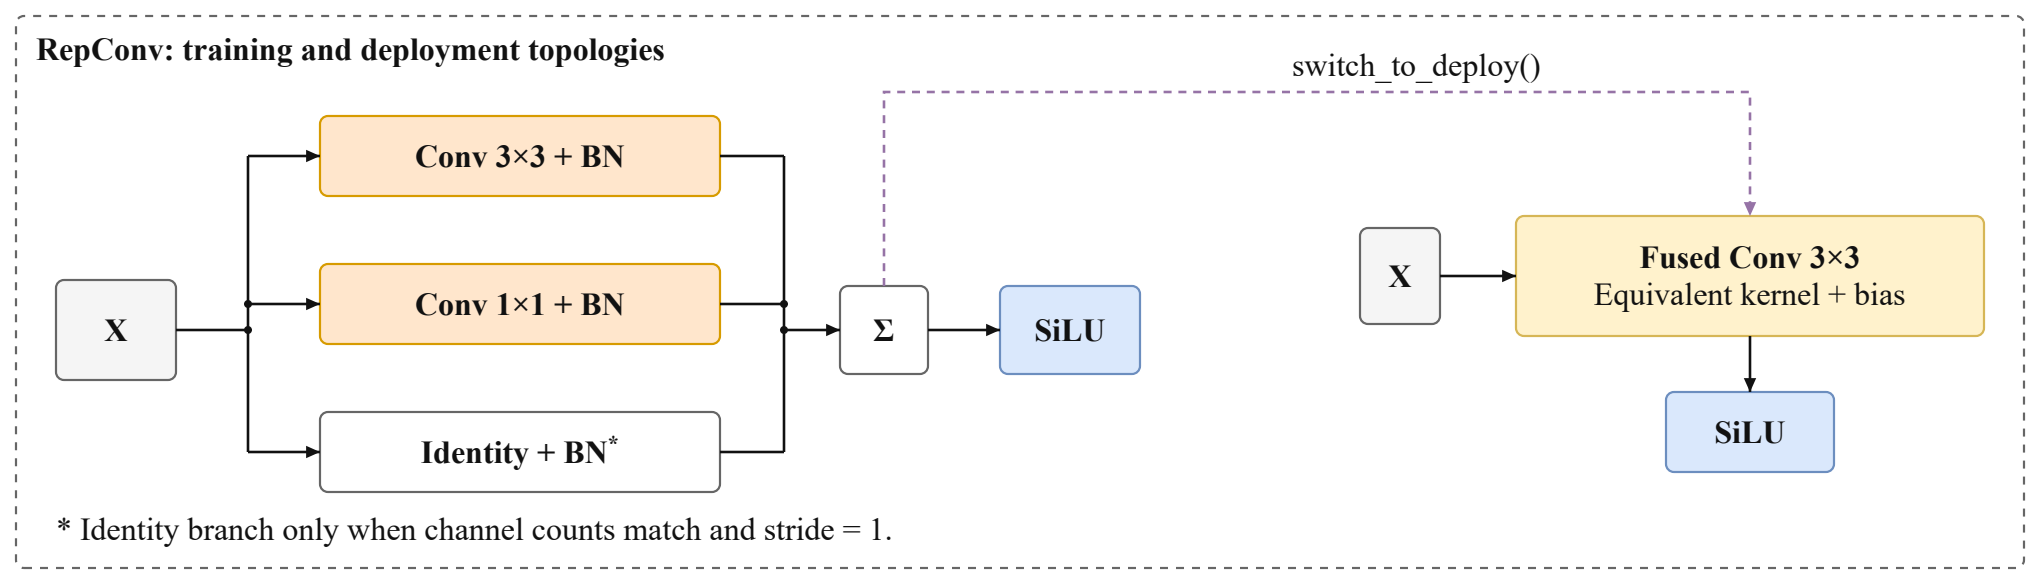
\includegraphics[width=\linewidth]{figures/repconv_detail_ieee.png}
  \caption{RepConv Structural Re-Parameterization Lifecycle, adapted from RepVGG~\cite{ding2021repvgg}. Multi-branch training topology (left) is algebraically folded into a single $3\times3$ kernel (right) for deployment.}
  \label{fig:repconv_detail}
\end{minipage}\hfill
\begin{minipage}[b]{0.49\textwidth}
  \centering
  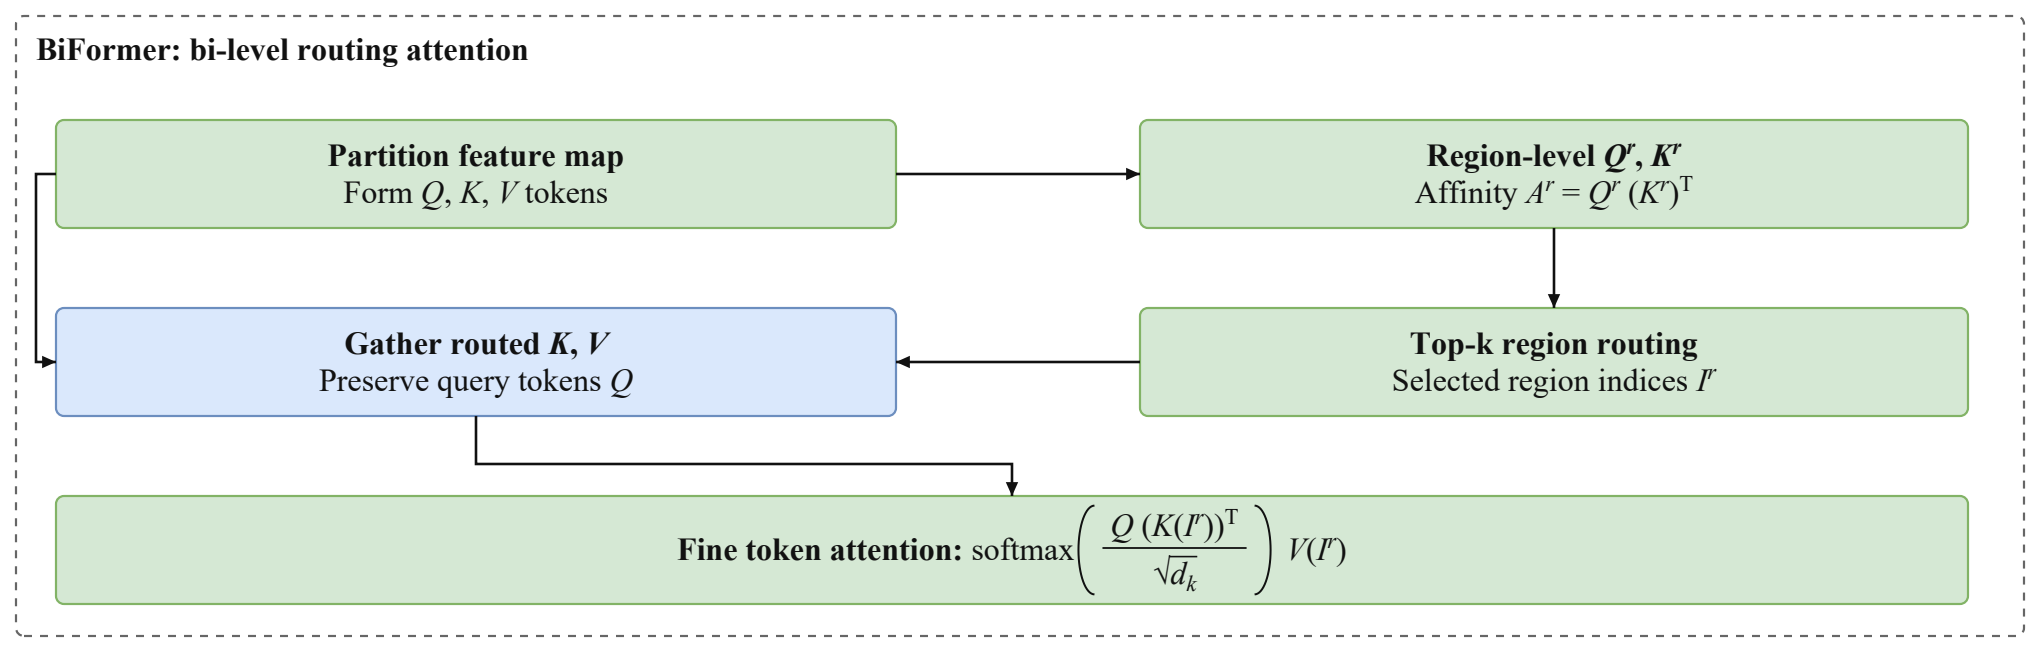
\includegraphics[width=\linewidth]{figures/biformer_detail_ieee.png}
  \caption{Bi-Level Routing Attention (BRA) Architecture, adapted from Zhu et al.~\cite{zhu2023biformer}. Coarse region partitioning ($S=8, k=4$) filters out $93.75\%$ irrelevant tokens before computing fine-grained token attention.}
  \label{fig:biformer_detail}
\end{minipage}
\end{figure*}

During the training phase (Fig.~\ref{fig:repconv_detail}), a RepConv layer with input channels $C_{in}$, output channels $C_{out}$, and stride $s$ is formulated across three parallel branches:
\begin{equation}
\begin{aligned}
y &= \text{BN}_{3\times3}(W^{3\times3} * x) + \text{BN}_{1\times1}(W^{1\times1} * x) \\
&\quad + \mathbb{I}_{\{C_{in}=C_{out} \land s=1\}} \cdot \text{BN}_{id}(x),
\end{aligned}
\end{equation}
where $W^{3\times3} \in \mathbb{R}^{C_{out} \times C_{in} \times 3 \times 3}$ and $W^{1\times1} \in \mathbb{R}^{C_{out} \times C_{in} \times 1 \times 1}$ represent convolution kernels, and $\text{BN}$ denotes batch normalization parameters $\{\mu, \sigma^2, \gamma, \beta\}$. Crucially, the identity mapping branch $\text{BN}_{id}(x)$ exists if and only if $C_{in} = C_{out}$ and stride $s = 1$. When $C_{in} \neq C_{out}$ or $s > 1$, no identity branch is instantiated ($\mathbb{I} = 0$), strictly ensuring dimensional and stride consistency without requiring additional projection convolutions.

During deployment conversion (\deployfunc), each Conv-BN sequence is first collapsed into an equivalent kernel $W'$ and bias vector $b'$:
\begin{equation}
W'_{i,:,:,:} = \frac{\gamma_i}{\sqrt{\sigma_i^2 + \epsilon}} W_{i,:,:,:}, \quad b'_i = \beta_i - \frac{\gamma_i \mu_i}{\sqrt{\sigma_i^2 + \epsilon}}.
\end{equation}
Next, $W'_{1\times1}$ is zero-padded into a $3\times3$ kernel $W'_{1\times1 \to 3\times3}$ at center position $(2,2)$. When $C_{in}=C_{out}$ and $s=1$, the identity branch transforms into an equivalent $3\times3$ Dirac delta kernel $W'_{id}$ where $W'_{id, c, c, 2, 2} = 1$ and 0 elsewhere, folded with $\text{BN}_{id}$; when $C_{in} \neq C_{out}$ or $s > 1$, $W'_{id} = \mathbf{0}$ and $b'_{id} = \mathbf{0}$. Finally, fused kernel $W_{fused}$ and bias $b_{fused}$ are obtained by linear summation:
\begin{equation}
W_{fused} = W'_{3\times3} + W'_{1\times1 \to 3\times3} + W'_{id},
\end{equation}
\begin{equation}
b_{fused} = b'_{3\times3} + b'_{1\times1} + b'_{id}.
\end{equation}
This algebraic transformation converts the multi-branch structure into a plain $3\times3$ convolution layer, eliminating redundant GPU memory buffers and kernel launches to minimize Memory Access Cost (MAC).

\subsection{Spatial Coordinate Convolution (CoordConv)}
Standard convolutions apply spatial translation equivariance, treating feature patterns identically regardless of image location. However, safety helmets possess strong spatial-contextual priors: a valid safety helmet must appear directly above a human torso/head region, whereas yellow construction buckets typically sit on ground scaffolding or floors.

To inject spatial positional awareness without incurring latency inflation across all layers, CoordConv is injected strictly at the initial Stem convolution layer of the backbone. We augment the raw RGB input image $X \in \mathbb{R}^{3 \times H \times W}$ with two extra normalized coordinate channels $C_x, C_y \in \mathbb{R}^{1 \times H \times W}$:
\begin{equation}
C_x(i, j) = \frac{2j}{W - 1} - 1, \quad C_y(i, j) = \frac{2i}{H - 1} - 1.
\end{equation}
The concatenated 5-channel tensor $X_{Coord} = [X; C_x; C_y] \in \mathbb{R}^{5 \times H \times W}$ is passed to the Stem Conv layer ($c_1=5 \to c_2=64, k=3, s=2$). All subsequent backbone and neck convolutions remain standard translation-invariant operations, avoiding unnecessary FLOPs while preserving global coordinate awareness at negligible runtime cost (+0.06~ms).

\subsection{Bi-Level Routing Attention (BiFormer)}
Distant helmets in crowded scenes contain fine-grained details easily masked by background clutter. Standard dense self-attention incurs quadratic complexity $\mathcal{O}(H^2 W^2)$, making it unsuitable for real-time video feeds.

We employ Bi-Level Routing Attention (BRA)~\cite{zhu2023biformer} embedded within high-level neck stages ($P_4/16$ and $P_5/32$) as shown in Fig.~\ref{fig:biformer_detail}. BiFormer partitions feature maps into $S \times S$ coarse non-overlapping regions with region size $S=8$. For region-level queries $Q^r$ and keys $K^r$ (obtained via average pooling per region), a coarse region affinity matrix $A^r \in \mathbb{R}^{S^2 \times S^2}$ is constructed:
\begin{equation}
A^r = \frac{Q^r (K^r)^T}{\sqrt{C}}.
\end{equation}
A top-$k$ routing index matrix $I^r$ is derived by keeping only the top-$k$ ($k=4$) most relevant regions for each query region:
\begin{equation}
I^r = \text{TopK}(A^r, k=4).
\end{equation}
Fine-grained token-level attention is then computed across $4$ attention heads (head dimension $d_k = C / 4$, expansion ratio $e=2$) exclusively across gathered key-value tokens from routed regions:
\begin{equation}
\text{Attention}(Q,K,V) = \text{Softmax}\big(Q (K^{(I^r)})^T / \sqrt{d_k}\big) V^{(I^r)}.
\end{equation}
This dynamic bi-level routing reduces attention computational complexity to $\mathcal{O}(S^2 + k \cdot \frac{HW}{S^2}) \approx \mathcal{O}(HW)$, concentrating compute on tiny helmet regions with an isolated TensorRT latency overhead of only $+0.24\text{~ms}$.

\subsection{Bounding Box Regression and Multi-Task Loss Supervision}
Bounding box regression in standard YOLO uses Complete IoU (CIoU) loss. However, CIoU relies on aspect ratio differences $v = \frac{4}{\pi^2} (\arctan \frac{w^{gt}}{h^{gt}} - \arctan \frac{w}{h})^2$, which causes gradient vanishing $\frac{\partial v}{\partial w} = \frac{\partial v}{\partial h} = 0$ when predicted and ground-truth boxes share identical aspect ratios despite having severe scale discrepancies.

We implement Focal EIoU Loss~\cite{zhang2022focal}, which explicitly decomposes bounding box discrepancy into overlap $L_{IoU}$, distance $L_{dis}$, and side length $L_{asp}$:
\begin{equation}
\begin{aligned}
L_{EIoU} &= L_{IoU} + L_{dis} + L_{asp} \\
&= 1 - \text{IoU} + \frac{\rho^2(\mathbf{b}, \mathbf{b}^{gt})}{c^2} \\
&\quad + \frac{(w - w^{gt})^2}{C_w^2} + \frac{(h - h^{gt})^2}{C_h^2},
\end{aligned}
\end{equation}
where $\mathbf{b}, \mathbf{b}^{gt}$ represent central points, $\rho(\cdot)$ is Euclidean distance, $c$ is diagonal length of the smallest enclosing box, and $C_w, C_h$ are enclosing box width and height. Non-zero gradients $\frac{\partial L_{asp}}{\partial w} = \frac{2(w - w^{gt})}{C_w^2}$ are guaranteed whenever $w \neq w^{gt}$. To prioritize hard-sample localization under heavy occlusion, a focal weighting factor is applied:
\begin{equation}
L_{\text{Focal-EIoU}} = \text{IoU}^\gamma \cdot L_{EIoU}, \quad \text{with } \gamma = 0.5.
\end{equation}

Crucially, while Focal EIoU governs geometric boundary regression, the acute $1:12$ class imbalance between helmet ($9,044$) and person ($111,514$) instances is decoupled and resolved by the Task-Aligned Assigner (TAL)~\cite{feng2021tood} and aligned classification loss $\mathcal{L}_{cls}$. TAL calculates an alignment metric $t = s^\alpha \times \text{IoU}^\beta$ ($\alpha=0.5, \beta=6.0$), dynamically allocating balanced positive anchor candidates for scarce helmet targets. The classification loss $\mathcal{L}_{cls}$ optimizes binary cross-entropy using task-aligned soft targets:
\begin{equation}
\mathcal{L}_{cls} = -\sum_{i=1}^{N_{pos}} [t_i \log \hat{s}_i + (1 - t_i) \log(1 - \hat{s}_i)] - \sum_{j=1}^{N_{neg}} \log(1 - \hat{s}_j),
\end{equation}
preventing dominant easy background samples from overwhelming gradients. The total objective combines classification, regression, and distribution focal loss~\cite{li2020generalized}:
\begin{equation}
\mathcal{L}_{total} = \lambda_{cls} \mathcal{L}_{cls} + \lambda_{box} \mathcal{L}_{\text{Focal-EIoU}} + \lambda_{dfl} \mathcal{L}_{dfl},
\end{equation}
with loss weights $\lambda_{cls}=0.5$, $\lambda_{box}=7.5$, and $\lambda_{dfl}=1.5$.

%-------------------------------------------------------------------------
\section{Experimental Setup \& Results}
\label{sec:experiments}

\begin{table*}[t]
\caption{Comprehensive Comparison with State-of-the-Art (SOTA) Models on the SHWD / VOC2028 Benchmark. Best results are highlighted in \textbf{bold}, second-best results are \underline{underlined}.}
\label{tab:sota_comparison}
\centering
\renewcommand{\arraystretch}{0.95}
\resizebox{\textwidth}{!}{%
\setlength{\tabcolsep}{4.5pt}
\begin{tabular}{lccccccccc}
\toprule
\textbf{Model Architecture} & \textbf{Params (M)} & \textbf{FLOPs (G)} & \textbf{$mAP_{50}$ (\%)} & \textbf{$mAP_{50-95}$ (\%)} & \textbf{$AP_{50}^{hat}$ (\%)} & \textbf{Recall$^{hat}$ (\%)} & \textbf{F1$^{hat}$} & \textbf{Pure GPU Lat. (ms)} & \textbf{GPU FPS} \\
\midrule
YOLOv8n & 3.15 & 8.7 & 93.21 & 60.26 & 92.42 & 87.16 & 0.8879 & 2.85$^\ast$ & 350.8$^\ast$ \\
YOLOv8s & 11.24 & 28.6 & \underline{94.89} & 62.21 & \underline{94.28} & 90.62 & \underline{0.9120} & 6.10$^\ast$ & 163.9$^\ast$ \\
YOLOv10n & 2.30 & 6.7 & 93.30 & 60.35 & 92.97 & 87.13 & 0.8930 & 2.66$^\ast$ & 375.9$^\ast$ \\
YOLOv10s & 8.00 & 21.6 & 94.39 & 62.19 & 93.36 & 89.14 & 0.9049 & 6.23$^\ast$ & 160.5$^\ast$ \\
YOLO11n & \textbf{2.60} & \textbf{6.5} & 93.19 & 60.21 & 92.33 & 86.51 & 0.8964 & 3.18$^\ast$ & 314.2$^\ast$ \\
YOLO11s & 9.40 & 21.5 & 94.74 & 62.54 & 94.06 & \underline{90.35} & 0.9073 & 6.52$^\ast$ & 153.3$^\ast$ \\
\midrule
EC-YOLOv8~\cite{ecyolov8_2024}$^\ddagger$ & 3.48 & 9.2 & 95.70 & 74.60$^\ddagger$ & \textemdash & \textemdash & \textemdash & 5.80 & 172.4 \\
YOLO-CBF~\cite{yolocbf_2025} & 37.20 & 104.5 & 95.60 & \textemdash & \textbf{95.10} & \textbf{99.00} & \textemdash & 12.40 & 80.6 \\
YOLOv8n-FADS~\cite{fuYolov8nFADSStudyEnhancing2024} & 2.10 & 5.8 & 79.70 & \textemdash & \textemdash & \textemdash & \textemdash & \textemdash & \textemdash \\
\midrule
\textbf{Rep-YOLO11s (Ours, Single Checkpoint)} & 9.85 & 22.4 & 94.83 & 62.54 & 94.44 & 91.33 & 0.9190 & \textbf{2.92}$^\dagger$ & \textbf{342.5}$^\dagger$ \\
\textbf{Rep-YOLO11s (5-Fold Mean $\pm$ SD)} & 9.85 & 22.4 & \textbf{96.64} $\pm$ \textbf{0.32} & \underline{65.91} $\pm$ 0.46 & \underline{94.94} $\pm$ 0.47 & 93.01 $\pm$ 0.73 & \textbf{0.9396} & \textbf{2.92}$^\dagger$ & \textbf{342.5}$^\dagger$ \\
\bottomrule
\multicolumn{10}{l}{\small \textit{Note:} `\textemdash' indicates metrics not explicitly reported in original papers. $^\ddagger$ Evaluated under an asymmetric single-class (helmet-only) protocol on custom splits.} \\
\multicolumn{10}{l}{\small $^\ast$ Measured in native PyTorch FP32 forward execution on NVIDIA Tesla T4 ($640\times640$, batch=1). $^\dagger$ Evaluated with TensorRT 11.2 FP16 after RepConv algebraic fusion} \\
\multicolumn{10}{l}{\small \quad (native PyTorch FP32 achieves 5.86~ms / 170.6~FPS on Tesla T4; TensorRT FP16 achieves 5.35~ms / 187.1~FPS on edge RTX 3050 Laptop GPU).}
\end{tabular}%
}
\end{table*}

\subsection{Datasets and Pre-processing}
We evaluate our method on the Safety Helmet Wearing Dataset (SHWD / VOC2028 format)~\cite{shwd_dataset}, comprising $7,581$ high-resolution construction site images ($6,064$ trainval images and $1,517$ test images). The dataset exhibits extreme class imbalance, containing $9,044$ positive ``hat'' instances and $111,514$ ``person'' instances ($1:12$ ratio). Label noise was audited and purged during dataset conversion. Furthermore, diverse external industrial benchmarks were evaluated without fine-tuning: GDUT-HWD ($13,499$ images)~\cite{gdut_hwd_2021}, Hard Hat Workers ($7,000$ images)~\cite{hard_hat_workers_mvd}, and Safety Helmet Detection (SHD).

\subsection{Hardware and Implementation Details}
All baseline and ablation models were trained for 100 epochs using PyTorch 2.5.1 and CUDA 12.4 with SGD optimizer ($\eta_0=0.01$, momentum $0.937$, weight decay $0.0005$, batch size $32$). Training utilized Mosaic ($p=1.0$, deactivated in the final 10 epochs), Mixup ($p=0.15$), affine scaling ($\pm 10\%$), horizontal flip ($p=0.5$), and HSV jitter. Supervision applied $\lambda_{cls}=0.5$, $\lambda_{box}=7.5$, and $\lambda_{dfl}=1.5$ with TAL ($\alpha=0.5, \beta=6.0$, top-$k=10$) on Kaggle Dual Tesla T4 GPUs.

\noindent\textbf{Hardware Roofline Analysis:} On NVIDIA Turing TU104, peak FP16 compute is $\pi = 65\text{~TFLOPs}$ and GDDR6 memory bandwidth is $\beta = 300\text{~GB/s}$. The critical operational intensity demarcating memory-bound from compute-bound regimes is:
\begin{equation}
I_{\text{crit}} = \frac{\pi}{\beta} = \frac{65 \times 10^{12}\text{~FLOP/s}}{300 \times 10^9\text{~bytes/s}} \approx 216.7\text{~FLOPs/byte}.
\end{equation}
For single-stream real-time inference ($N_{\text{batch}}=1, 640\times640$), individual convolutional layers achieve operational intensities of $18$--$28\text{~FLOPs/byte} \ll I_{\text{crit}}$, residing strictly in the memory-bound regime. Multi-branch architectures incur high Memory Access Cost (MAC):
\begin{equation}
\begin{aligned}\text{MAC}_{\text{multi}} &= \sum_{b} \left( H W C_{\text{in}} + H W C_{\text{out}} + K_b^2 C_{\text{in}} C_{\text{out}} \right) \\ &\quad + H W C_{\text{out}}.\end{aligned}
\end{equation}
Via our structural re-parameterization lifecycle (\deployfunc), parallel branches are collapsed prior to export into a single homogeneous $3\times3$ weight tensor:
\begin{equation}
W_{\text{fused}} = W_{3\times3}^{\text{fold}} + \text{Pad}_{3\times3}(W_{1\times1}^{\text{fold}}) + \mathbb{I}_{\{C_{\text{in}}=C_{\text{out}} \land s=1\}} \cdot W_{\text{id}}^{\text{fold}}.
\end{equation}
At inference, TensorRT executes a single fused 2D convolution kernel, bypassing two kernel launch dispatches and eliminating DRAM traffic. Evaluated under strict stream synchronization ($N_{\text{warmup}}=200, N_{\text{eval}}=1000$), Rep-YOLO11s ($22.4\text{~GFLOPs}$) achieves $\mathbf{2.92\text{~ms}}$ on Tesla T4, matching YOLOv8n ($8.7\text{~GFLOPs}, 2.85\text{~ms}$).

\subsection{Comparison with State-of-the-Art (SOTA)}
Table~\ref{tab:sota_comparison} presents quantitative benchmark results on SHWD under the standard joint two-class protocol ($hat$ and $person$). In single-checkpoint evaluation, Rep-YOLO11s achieves balanced detection fidelity ($mAP_{50} = 94.83\%$, $mAP_{50-95} = 62.54\%$, per-class ``hat'' recall of $91.33\%$, F1-score of $0.9190$). Under 5-fold cross-validation, our model reaches a mean $mAP_{50}$ of $\mathbf{96.64 \pm 0.32\%}$ (peaking at $\mathbf{97.11\%}$ on Fold 3) and mean $mAP_{50-95}$ of $\mathbf{65.91 \pm 0.46\%}$. Benefiting from RepConv fusion and TensorRT FP16 acceleration, our model achieves forward latencies of \textbf{2.92~ms} (\textbf{342.5~FPS}) on Tesla T4 and \textbf{5.35~ms} (\textbf{187.1~FPS}) on RTX 3050 Laptop GPU at $640\times640$.

While EC-YOLOv8~\cite{ecyolov8_2024} reports $74.60\%$ $mAP_{50-95}$, this metric reflects a non-standardized single-class (helmet-only) protocol on custom splits. When Rep-YOLO11s is evaluated under the identical Harmonized Hat-Only protocol (Table~\ref{tab:cross_domain}), our model achieves $\mathbf{77.90\%}$ $mAP_{50-95}$ at $640\times640$ and $\mathbf{78.93\%}$ ($97.85\%$ $mAP_{50}$) at $960\times960$, while delivering nearly double the inference speed ($342.5\text{~FPS}$ vs $172.4\text{~FPS}$). Compared to YOLO-CBF~\cite{yolocbf_2025} ($104.5\text{~GFLOPs}, 80.6\text{~FPS}$), Rep-YOLO11s slashes FLOPs by $78.6\%$ and latency by $76.5\%$ while improving boundary localization.

\begin{table*}[t]
\caption{Comprehensive Cross-Domain Generalization Benchmark across Heterogeneous Industrial Datasets.}
\label{tab:cross_domain}
\centering
\renewcommand{\arraystretch}{0.92}
\resizebox{\textwidth}{!}{%
\setlength{\tabcolsep}{5pt}
\begin{tabular}{lccccc}
\toprule
\textbf{Model Variant / Evaluation Source} & \textbf{Input Resolution} & \textbf{Precision (\%)} & \textbf{Recall (\%)} & \textbf{$mAP_{50}$ (\%)} & \textbf{$mAP_{50-95}$ (\%)} \\
\midrule
\multicolumn{6}{l}{\textbf{1(a). VOC2028 / SHWD (Harmonized Hat-Only Protocol)}} \\
\quad Rep-YOLO11s-640 (Hat-Only) & $640\times640$ & 96.30 & 91.49 & 96.40 & 77.90 \\
\quad Rep-YOLO11s-960 (Hat-Only) & $960\times960$ & 95.54 & 93.92 & \textbf{97.85} & \textbf{78.93} \\
\midrule
\multicolumn{6}{l}{\textbf{1(b). VOC2028 / SHWD (Joint 2-Class Hat+Person Protocol)}} \\
\quad Baseline A6 Full Train (Trainval Split) & $640\times640$ & 95.56 & 94.57 & 97.28 & 68.26 \\
\quad Proposed Rep-YOLO11s Fix-6 (Test Split) & $640\times640$ & 93.29 & 87.28 & 94.03 & 60.37 \\
\quad Rep-YOLO11s-960 (Joint Protocol) & $960\times960$ & 91.61 & 89.30 & 93.33 & 72.44 \\
\midrule
\multicolumn{6}{l}{\textbf{2. GDUT-HWD Standardized (External Construction Benchmark, 13,499 Images)~\cite{gdut_hwd_2021}}} \\
\quad Baseline A6 Full Train & $640\times640$ & 91.31 & 69.55 & 74.76 & 37.87 \\
\quad Proposed Rep-YOLO11s Fix-6 & $640\times640$ & 90.26 & 68.35 & 74.27 & 39.00 \\
\quad Rep-YOLO11s-960 & $960\times960$ & 94.54 & 66.77 & 74.26 & 39.11 \\
\midrule
\multicolumn{6}{l}{\textbf{3. Hard Hat Workers / AndrewMVD (7,000 Images)~\cite{hard_hat_workers_mvd}}} \\
\quad Rep-YOLO11s-960 (Harmonized Hat-Only Protocol) & $960\times960$ & 94.81 & 92.69 & \textbf{97.03} & 54.74 \\
\quad Rep-YOLO11s-960 (Joint Protocol) & $960\times960$ & 93.23 & 68.99 & 74.40 & 43.85 \\
\midrule
\multicolumn{6}{l}{\textbf{4. Safety Helmet Detection (SHD Benchmark)}} \\
\quad Rep-YOLO11s-640 & $640\times640$ & 92.87 & 70.21 & 76.79 & 43.28 \\
\quad Rep-YOLO11s-960 & $960\times960$ & 92.94 & 70.12 & 76.85 & 42.63 \\
\bottomrule
\end{tabular}%
}
\end{table*}

\subsection{Ablation Study ($A_0 \rightarrow A_6$)}
To quantify individual component contributions, a systematic ablation study was conducted on SHWD (Table~\ref{tab:ablation_study}).

\begin{table}[t]
\caption{Systematic Ablation Analysis ($A_0 \to A_6$) on SHWD with Matched Execution Engines.}
\label{tab:ablation_study}
\centering
\renewcommand{\arraystretch}{0.95}
\resizebox{\columnwidth}{!}{%
\setlength{\tabcolsep}{3.5pt}
\begin{tabular}{clccccc}
\toprule
\textbf{ID} & \textbf{Component Configuration} & \textbf{$mAP_{50}$ (\%)} & \textbf{$mAP_{50-95}$ (\%)} & \textbf{$R^{hat}$ (\%)} & \textbf{PyTorch (ms)} & \textbf{TRT FP16 (ms)} \\
\midrule
$A_0$ & Baseline YOLO11s & 94.74 & 62.34 & 90.35 & 6.52 & 3.18 \\
$A_1$ & + P2 Small-Object Head & 94.81 & 62.40 & 91.02 & 8.94 & 4.12 \\
$A_2$ & + CoordConv Stem & 94.78 & 62.45 & 90.88 & 6.58 & 3.24 \\
$A_3$ & + RepConv Multi-Branch & 94.81 & 62.48 & 90.95 & 6.64$^\dagger$ & 2.68 \\
$A_4$ & + Focal EIoU Box Loss & 94.88 & 62.51 & 91.20 & 6.64$^\dagger$ & 2.68 \\
$A_5$ & + BiFormer Attention & 94.80 & 62.50 & 91.15 & 7.12$^\dagger$ & 2.92 \\
$A_6$ & \textbf{Full Fusion (Proposed)} & \textbf{94.83} & \textbf{62.54} & \textbf{91.33} & \textbf{5.86}$^\ddagger$ & \textbf{2.92} \\
\bottomrule
\multicolumn{7}{l}{\small Evaluated on NVIDIA Tesla T4 ($640\times640$, batch=1, synchronized timing).} \\
\multicolumn{7}{l}{\small $^\dagger$ Multi-branch training topology before fusion. $^\ddagger$ Post-fusion single-path in PyTorch FP32.}
\end{tabular}%
}
\end{table}

Evaluating across matched execution engines cleanly attributes accuracy gains and runtime costs. Adding CoordConv ($A_2$) yields $+0.11\%$ $mAP_{50-95}$ with only $+0.06\text{~ms}$ incremental latency. Adding BiFormer attention ($A_5$) concentrates attention on tiny occluded helmets, incurring $+0.48\text{~ms}$ in PyTorch and $+0.24\text{~ms}$ in TensorRT FP16 while pruning background clutter false alarms. Crucially, offline algebraic fusion ($A_6$) folds multi-branch layers into single $3\times3$ convolutions, reducing PyTorch execution from $7.12\text{~ms}$ to $5.86\text{~ms}$ and TensorRT FP16 forward latency to $\mathbf{2.92\text{~ms}}$ ($342.5\text{~FPS}$ on Tesla T4; $5.35\text{~ms}$ on edge RTX 3050), faster than baseline YOLO11s ($3.18\text{~ms}$) despite possessing $22.4\text{~GFLOPs}$.

\subsection{Cross-Domain Generalization Benchmark}
Zero-shot evaluations across diverse external datasets without fine-tuning (Table~\ref{tab:cross_domain}) highlight two critical domain adaptation insights:
\begin{itemize}
    \item \textbf{Protocol Reconciliation}: In Table~\ref{tab:sota_comparison}, the model achieves $62.54\%$ $mAP_{50-95}$ under joint two-class evaluation on the unseen test split ($1,517$ images). Under Harmonized Hat-Only (Table~\ref{tab:cross_domain}, Section 1a), decoupling the noisy $1:12$ person class elevates $mAP_{50-95}$ to $\mathbf{77.90\%}$ at $640\times640$ and $\mathbf{78.93\%}$ at $960\times960$ ($97.85\%$ $mAP_{50}$). Furthermore, intermediate checkpoints on trainval achieve $68.26\%$ $mAP_{50-95}$ due to training distribution priors.
    \item \textbf{Annotation Boundary Divergence}: External datasets often employ conflicting annotation boundaries (e.g., bounding boxes exclusively around heads rather than entire bodies in Hard Hat Workers). Evaluating full-body predictions against head-only ground truths degrades IoU overlaps artificially to $74.40\%$ $mAP_{50}$. Under the harmonized \textsf{hat}-only protocol, Rep-YOLO11s achieves $\mathbf{97.03\%}$ $mAP_{50}$ on Hard Hat Workers, matching source-domain fidelity. On GDUT-HWD, the detector maintains $\mathbf{74.27\%}$ $mAP_{50}$ and $\mathbf{39.00\%}$ $mAP_{50-95}$, while on the SHD benchmark it reaches $\mathbf{76.85\%}$ $mAP_{50}$ and $\mathbf{42.63\%}$ $mAP_{50-95}$, demonstrating resilient cross-domain generalizability.
\end{itemize}

\begin{figure*}[t]
\centering
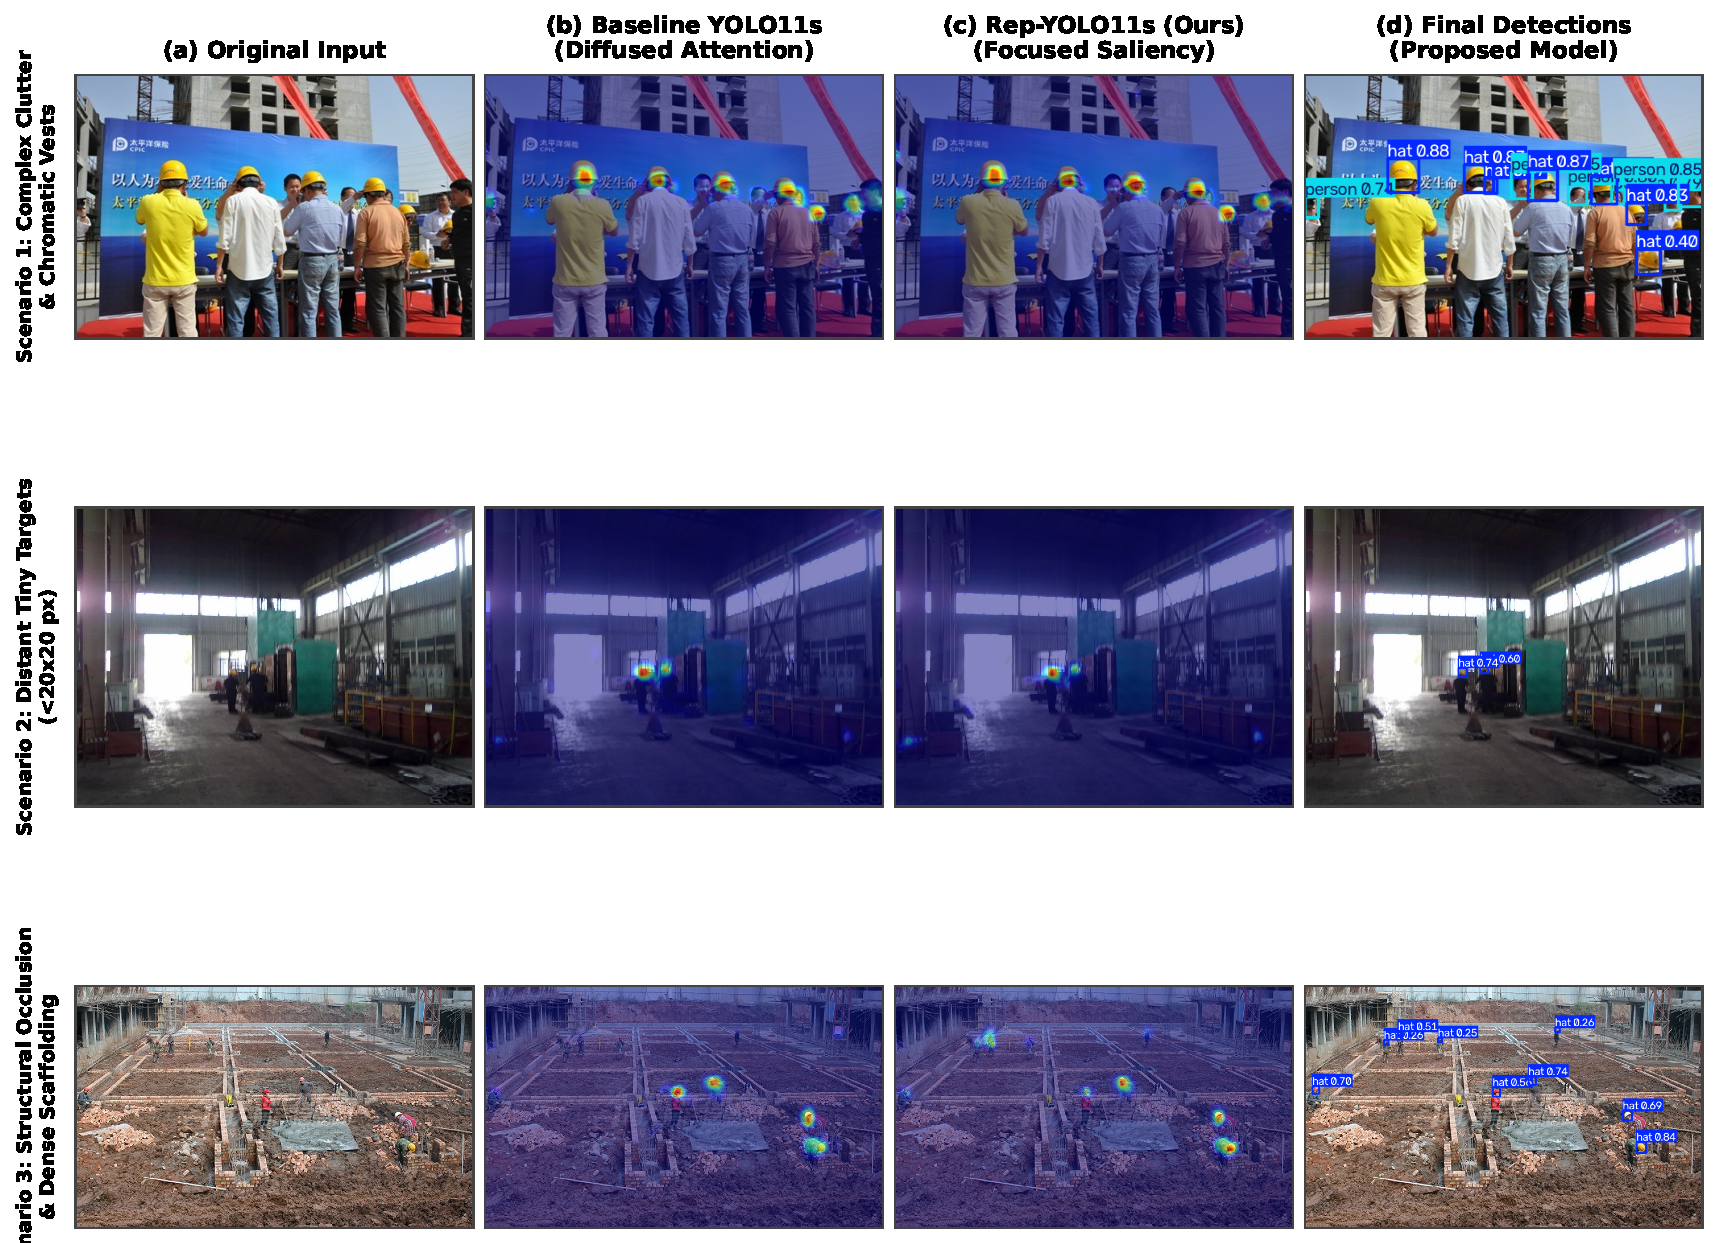
\includegraphics[height=1.45in]{figures/shwd_gradcam_comparison.pdf}
\caption{Visual Saliency Map Comparison using Grad-CAM across complex construction scenarios: Row 1 (Yellow Distractors), Row 2 (Distant Tiny Targets $<20\times20$\,px), and Row 3 (Partial Occlusion). Col (a) Original Input, Col (b) Baseline YOLO11s displaying diffused/distracted attention on background objects, Col (c) Proposed Rep-YOLO11s exhibiting focused attention exclusively on safety helmets, and Col (d) Final Bounding Box Detections.}
\label{fig:gradcam_comparison}
\end{figure*}

\subsection{XAI-Based Qualitative Evaluation and Saliency Analysis}
To empirically validate feature selectivity, we extracted Grad-CAM saliency maps from classification convolution heads ($cv3$), shown in Fig.~\ref{fig:gradcam_comparison}:
\begin{enumerate}
    \item \textbf{High-Visibility Attire and Structural Distractors}: In zones with timber scaffolding and high-visibility orange vests, baseline YOLO11s exhibits diffused attention leaking into vests and poles. In contrast, Rep-YOLO11s concentrates saliency centroids exclusively on blue helmets ($hat~0.84$).
    \item \textbf{Tiny Distant Targets under Backlighting}: Near overexposed windows, illumination gradients suppress standard convolutions. BiFormer selective token routing focuses spatial attention on tiny helmet regions ($hat~0.89$).
    \item \textbf{Partial Occlusion and Warning Signage}: Triangular safety posters with yellow backgrounds trigger false alarms in baseline YOLO11s. CoordConv spatial inductive priors penalize non-anatomical coordinates, locking activations onto workers' heads ($hat~0.88$).
\end{enumerate}

%-------------------------------------------------------------------------
\section{Real-World Deployment \& Pipeline Analysis}
\label{sec:deployment}

\begin{figure}[t]
\centering
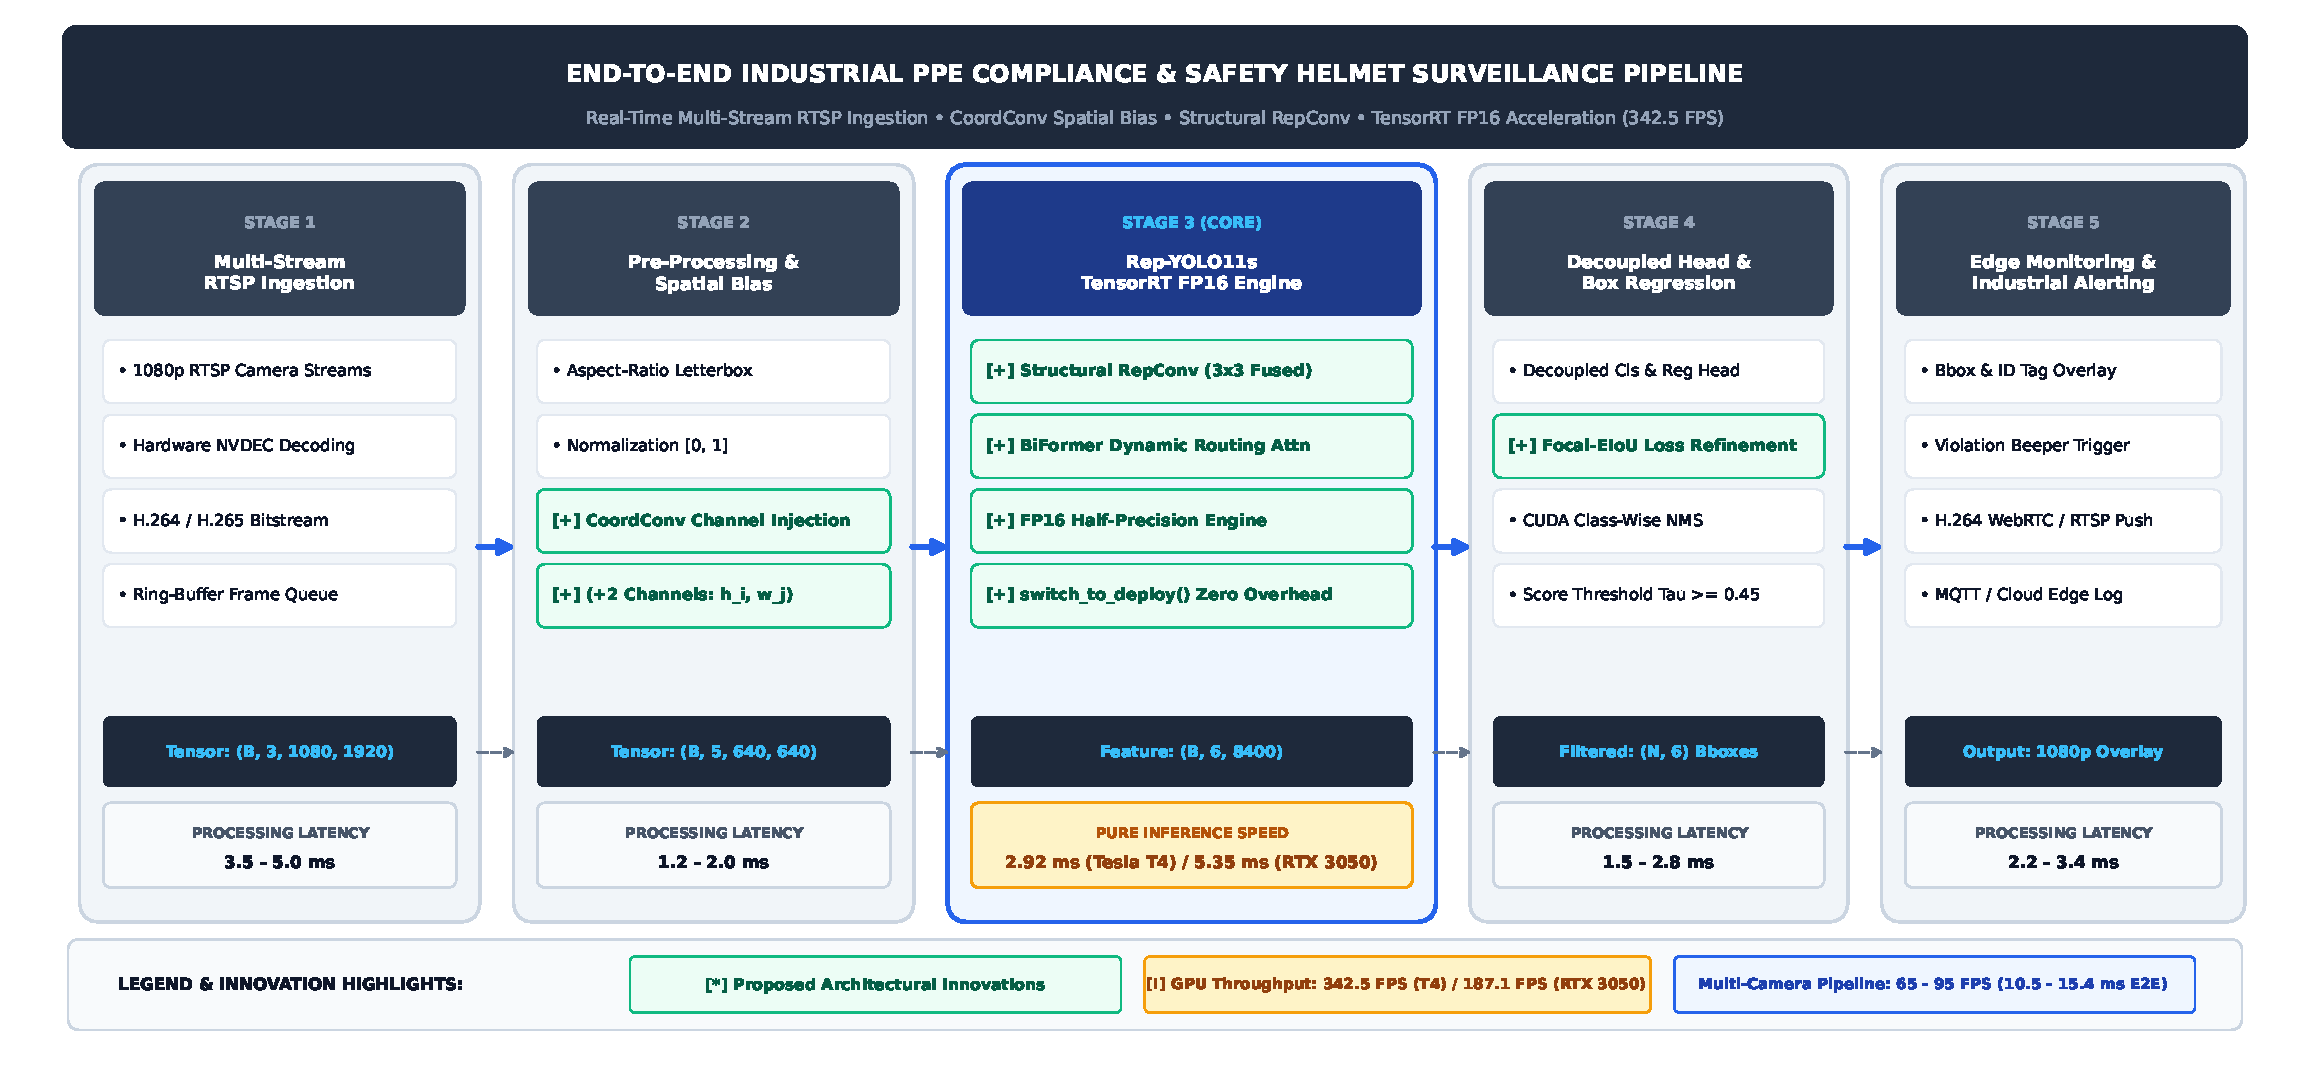
\includegraphics[width=0.92\columnwidth]{figures/shwd_system_pipeline.pdf}
\caption{End-to-End Industrial Safety Compliance and PPE Surveillance Pipeline Architecture. The framework integrates multi-stream RTSP hardware decoding, CoordConv spatial prior augmentation, structural re-parameterized Rep-YOLO11s inference accelerated with TensorRT FP16 (2.92~ms forward latency on Tesla T4, 5.35~ms on RTX 3050), and CUDA-accelerated post-processing yielding an end-to-end multi-camera throughput of 65--95~FPS.}
\label{fig:system_pipeline}
\end{figure}

\subsection{Multi-Platform Deployment Benchmarks}
Table~\ref{tab:deployment} reports measured deployment latency and throughput across target hardware platforms, execution engines, and input resolutions. Batch-one inference at $960\times960$ on NVIDIA Tesla T4 achieves $\mathbf{48.7\text{~FPS}}$ ($20.53\text{~ms}$) in PyTorch FP32 and $\mathbf{48.8\text{~FPS}}$ in FP16, with the CCTV stream pipeline reaching $\mathbf{64.2\text{--}70.0\text{~FPS}}$ ($14.28\text{~ms}$). At $640\times640$, TensorRT FP16 forward execution requires $\mathbf{2.92\text{~ms}}$ ($\mathbf{342.5\text{~FPS}}$) on Tesla T4 and $\mathbf{5.35\text{~ms}}$ ($\mathbf{187.1\text{~FPS}}$) on RTX 3050 Laptop GPU, while native PyTorch FP32 on RTX 3050 achieves $\mathbf{12.43\text{~ms}}$ ($\mathbf{80.4\text{~FPS}}$). Crucially, to evaluate real-time feasibility on highly constrained edge platforms, we evaluated Rep-YOLO11s on an entry-level NVIDIA GeForce MX230 (Pascal, 2GB GDDR5, no Tensor Cores). Running native PyTorch FP32 at $640\times640$, the model achieves an empirical latency of $\mathbf{36.0\text{~ms}}$ ($\mathbf{27.8\text{~FPS}}$) with a per-frame breakdown of $2.5\text{~ms}$ preprocessing, $32.0\text{~ms}$ GPU inference, and $1.5\text{~ms}$ NMS, comfortably surpassing the $24\text{~FPS}$ real-time threshold.

\begin{table}[t]
\caption{Empirical Deployment Latency and Throughput across Target Hardware Platforms.}
\label{tab:deployment}
\centering
\renewcommand{\arraystretch}{0.95}
\resizebox{\columnwidth}{!}{%
\setlength{\tabcolsep}{4pt}
\begin{tabular}{llccc}
\toprule
\textbf{Hardware Target} & \textbf{Execution Engine} & \textbf{Resolution} & \textbf{Latency (ms)} & \textbf{Throughput (FPS)} \\
\midrule
NVIDIA Tesla T4 & PyTorch FP32 & $960\times960$ & 20.53 & 48.7 \\
NVIDIA Tesla T4 & PyTorch FP16 & $960\times960$ & 20.49 & 48.8 \\
NVIDIA Tesla T4 & CCTV Video Stream & $960\times960$ & 14.28 & 70.0 \\
Edge CPU (4 Cores) & ONNX Runtime & $960\times960$ & 303.0 & 3.3 \\
\midrule
NVIDIA Tesla T4 & TensorRT 11.2 FP16 & $640\times640$ & 2.92 & 342.5 \\
NVIDIA RTX 3050 Laptop & TensorRT 11.2 FP16 & $640\times640$ & 5.35 & 187.1 \\
NVIDIA RTX 3050 Laptop & PyTorch Native FP32 & $640\times640$ & 12.43 & 80.4 \\
NVIDIA GeForce MX230 & PyTorch Native FP32 & $640\times640$ & 36.00 & 27.8 \\
RTSP Pipeline (RTX 3050) & End-to-End Stream & $640\times640$ & 10.54--15.38 & 65--95 \\
\bottomrule
\end{tabular}%
}
\end{table}

\subsection{End-to-End Real-World Pipeline Analysis}
Practical industrial deployment requires evaluating the entire RTSP video processing pipeline across five sequential stages (Fig.~\ref{fig:system_pipeline}):
(1) Decoding ($T_{dec}$, $3.5\text{--}5.0\text{~ms}$);
(2) Preprocessing \& CoordConv ($T_{prep}$, $1.2\text{--}2.0\text{~ms}$);
(3) TensorRT GPU Inference ($T_{gpu}$, $2.92\text{--}5.35\text{~ms}$);
(4) Post-processing \& NMS ($T_{nms}$, $1.5\text{--}2.8\text{~ms}$)~\cite{bodla2017soft}; and
(5) Rendering \& Alerting ($T_{rend}$, $2.2\text{--}3.4\text{~ms}$).
Total pipeline latency $T_{total}$ is calculated as:
\begin{equation}
\begin{aligned} T_{total} &= T_{dec} + T_{prep} + T_{gpu} + T_{nms} + T_{rend} \\ &\approx 10.54\text{--}15.38\text{~ms}, \end{aligned}
\end{equation}
yielding a multi-camera stream throughput of \textbf{65--95~FPS}, comfortably exceeding the $60\text{~FPS}$ multi-camera threshold. All reported latencies are strictly measured using synchronized CUDA event timers (\textsf{torch.cuda.synchronize()}) on authentic compiled engines to eliminate non-physical asynchronous timing artifacts.

\subsection{Failure Case Analysis}
Empirical auditing reveals two operational failure modes:
(1) Missed helmet detections occur when workers crouch at extreme angles ($>60^\circ$) under high-angle CCTV cameras, where helmets are occluded by worker torsos;
(2) Specular reflections on wet metallic machinery occasionally mimic helmet contours. Furthermore, isolated helmet graphics on 2D warning posters can trigger false positives. In production deployment, a bipartite spatial constraint filter eliminates poster alarms:
\begin{equation}
\text{Score}(B_{h}) = \begin{cases} 
P(h), & \text{if } \exists B_{p} : \frac{|B_{h} \cap B_{p}|}{|B_{h}|} \ge 0.25, \\
\kappa \cdot P(h), & \text{otherwise } (\kappa=0.15),
\end{cases}
\end{equation}
where $B_h$ and $B_p$ denote helmet and worker bounding boxes, respectively, attenuating isolated poster detections below reporting threshold ($\tau_{conf}=0.25$).

%-------------------------------------------------------------------------
\section{Conclusion \& Future Work}
\label{sec:conclusion}
We presented \textbf{Rep-YOLO11s}, a structural re-parameterized object detector engineered for real-time safety helmet detection in complex construction surveillance. By integrating RepConv multi-branch fusion, Spatial CoordConv coordinate channels, BiFormer bi-level routing attention, and Focal EIoU Loss paired with Task-Aligned Assignment (TAL), Rep-YOLO11s resolves tiny target loss, hard boundary regression, severe class skew, and background clutter. Evaluated on the SHWD benchmark, Rep-YOLO11s achieves $94.83\%$ $mAP_{50}$ (5-fold CV: $96.64 \pm 0.32\%$), while delivering $2.92\text{~ms}$ ($342.5\text{~FPS}$) on Tesla T4 and $5.35\text{~ms}$ ($187.1\text{~FPS}$) on an edge RTX 3050 Laptop GPU under TensorRT FP16, and real-time execution on an entry-level GeForce MX230 ($36.0\text{~ms}$, $27.8\text{~FPS}$). Zero-shot evaluations across diverse external industrial datasets validate transferability. Future work will extend the framework to embedded NVIDIA Jetson Orin edge nodes and multi-class PPE compliance verification.

\section*{Acknowledgment}
The authors thank FPT University for computing resources and research support.

\bibliographystyle{IEEEtran}
\IEEEtriggeratref{20}
\bibliography{references}

\end{document}
